\chapter{Introduction}
\label{chpt:introduction}

% explain the core SAC signaling cascade vs RZZ pathway: An unattached kinetochore activates the SAC by allowing Mps1 kinase to phosphorylate KNL1 at sites known as MELT motifs due to their consensus sequence (Figures 1B and 1C) [7–10]. This event is followed by the sequential recruitment of Bub3-Bub1 and Mad1-Mad2, along with Bub3-BubR1 and Cdc20 to the kinetochore, with Mps1 phosphorylation playing a licensing role for each step (Figure 1B) [2, 11–19]. We refer to this biochemical cascade as the ‘‘core SAC signaling cascade’’ (dashed gray box in Figure 1B). In metazoa, the core SAC signaling cascade is complemented by the RZZ pathway, which independently recruits additional Mad1-Mad2 to the kinetochore [20]. Ultimately, Bub3, BubR1, Mad2, and Cdc20 form the MCC, which then disperses throughout the cellular volume to inhibit APC/C.

% Accurate chromosome segregation during cell division requires that the sister kinetochores on each replicated chromosome are stably attached to microtubules emanating from opposite spindle poles before the cell divides. If one or more kinetochores fail to attach to microtubules, they activate a biochemical signaling cascade known as the spindle assembly checkpoint (SAC). This cascade produces an anaphase-inhibitory signal known as the ‘‘mitotic checkpoint complex’’ (MCC). MCC in- hibits the anaphase promoting complex/cyclosome (APC/C) to prevent the cell from transitioning from prometaphase to anaphase, thus avoiding chromosome mis-segregation [2].

% The kinetochore-localized signaling activity of tightly clustered \protein{Knl1} molecules.

\begin{figure}
    \centering
    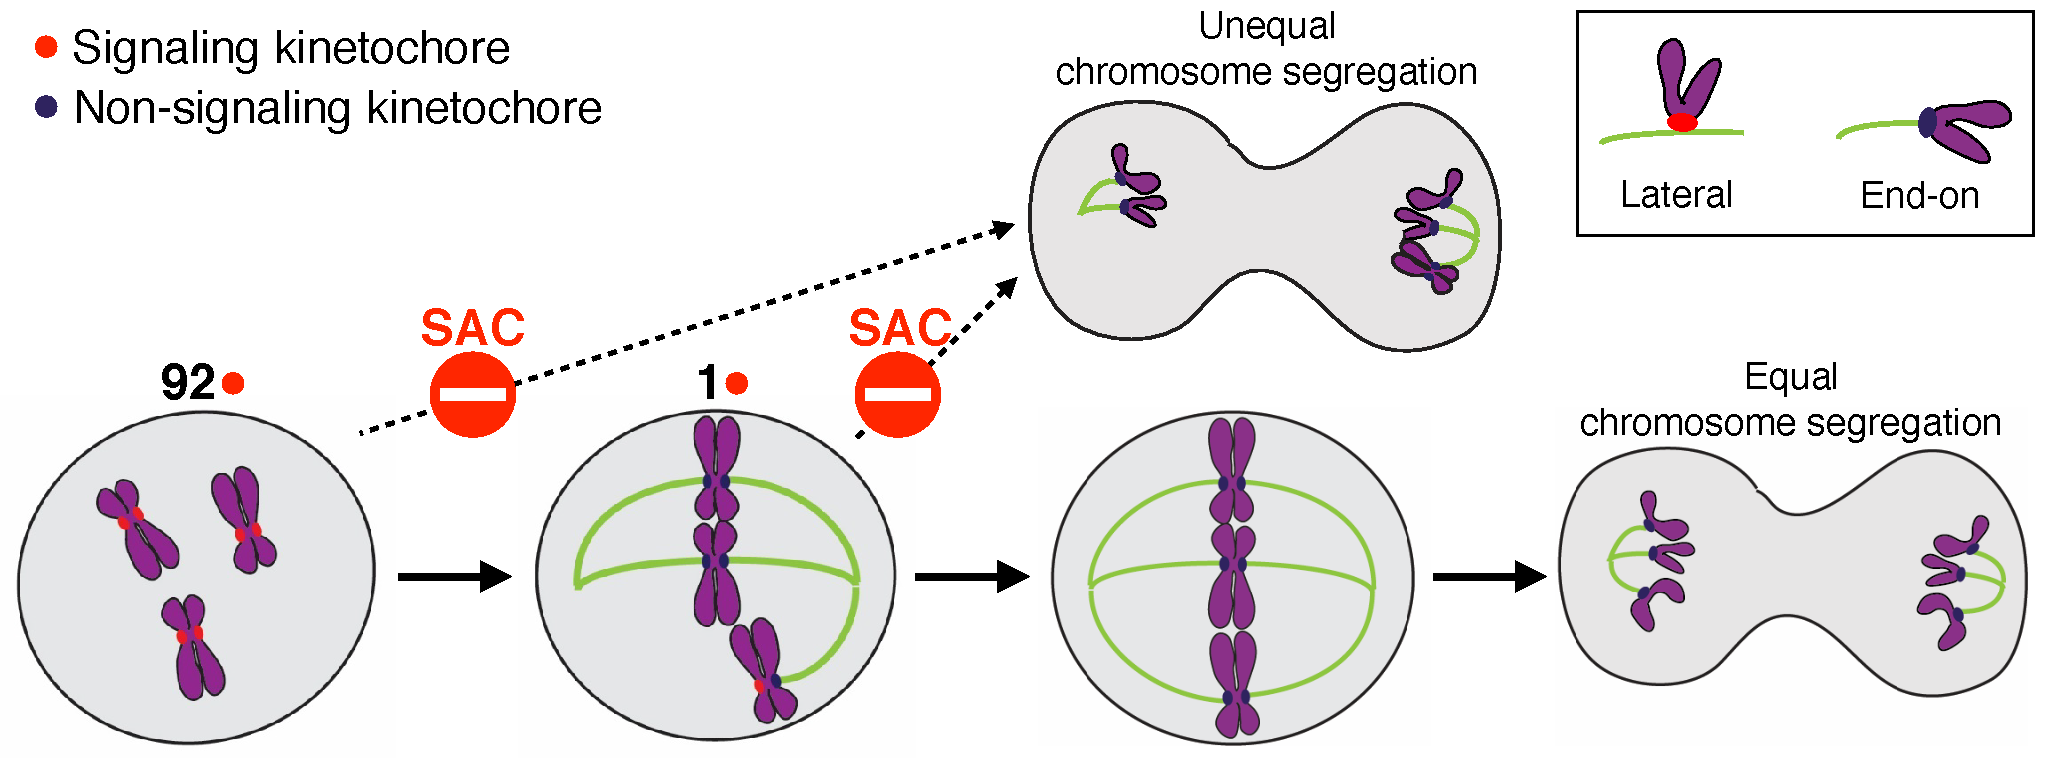
\includegraphics[width=0.95\textwidth]{chapters/figures/SACRole.pdf}
    \caption{\textbf{A diagram illustrating the role and properties of the spindle assembly checkpoint (SAC).}}
    \label{SACRole}
\end{figure}